\begin{figure}[htbp]
\centering
\captionsetup{justification=raggedright,labelsep=none,singlelinecheck=false,labelformat=boldlabel}
\caption[Productivity of the reviewed literature]{\footnotesize \textbf{: Productivity of the reviewed literature.} Panel (a) reports the fifteen sources publishing the most articles in the review set. Panel (b) reports the fifteen most frequent corresponding-author countries. Long source names are truncated.}
\begin{subfigure}{\linewidth}\centering
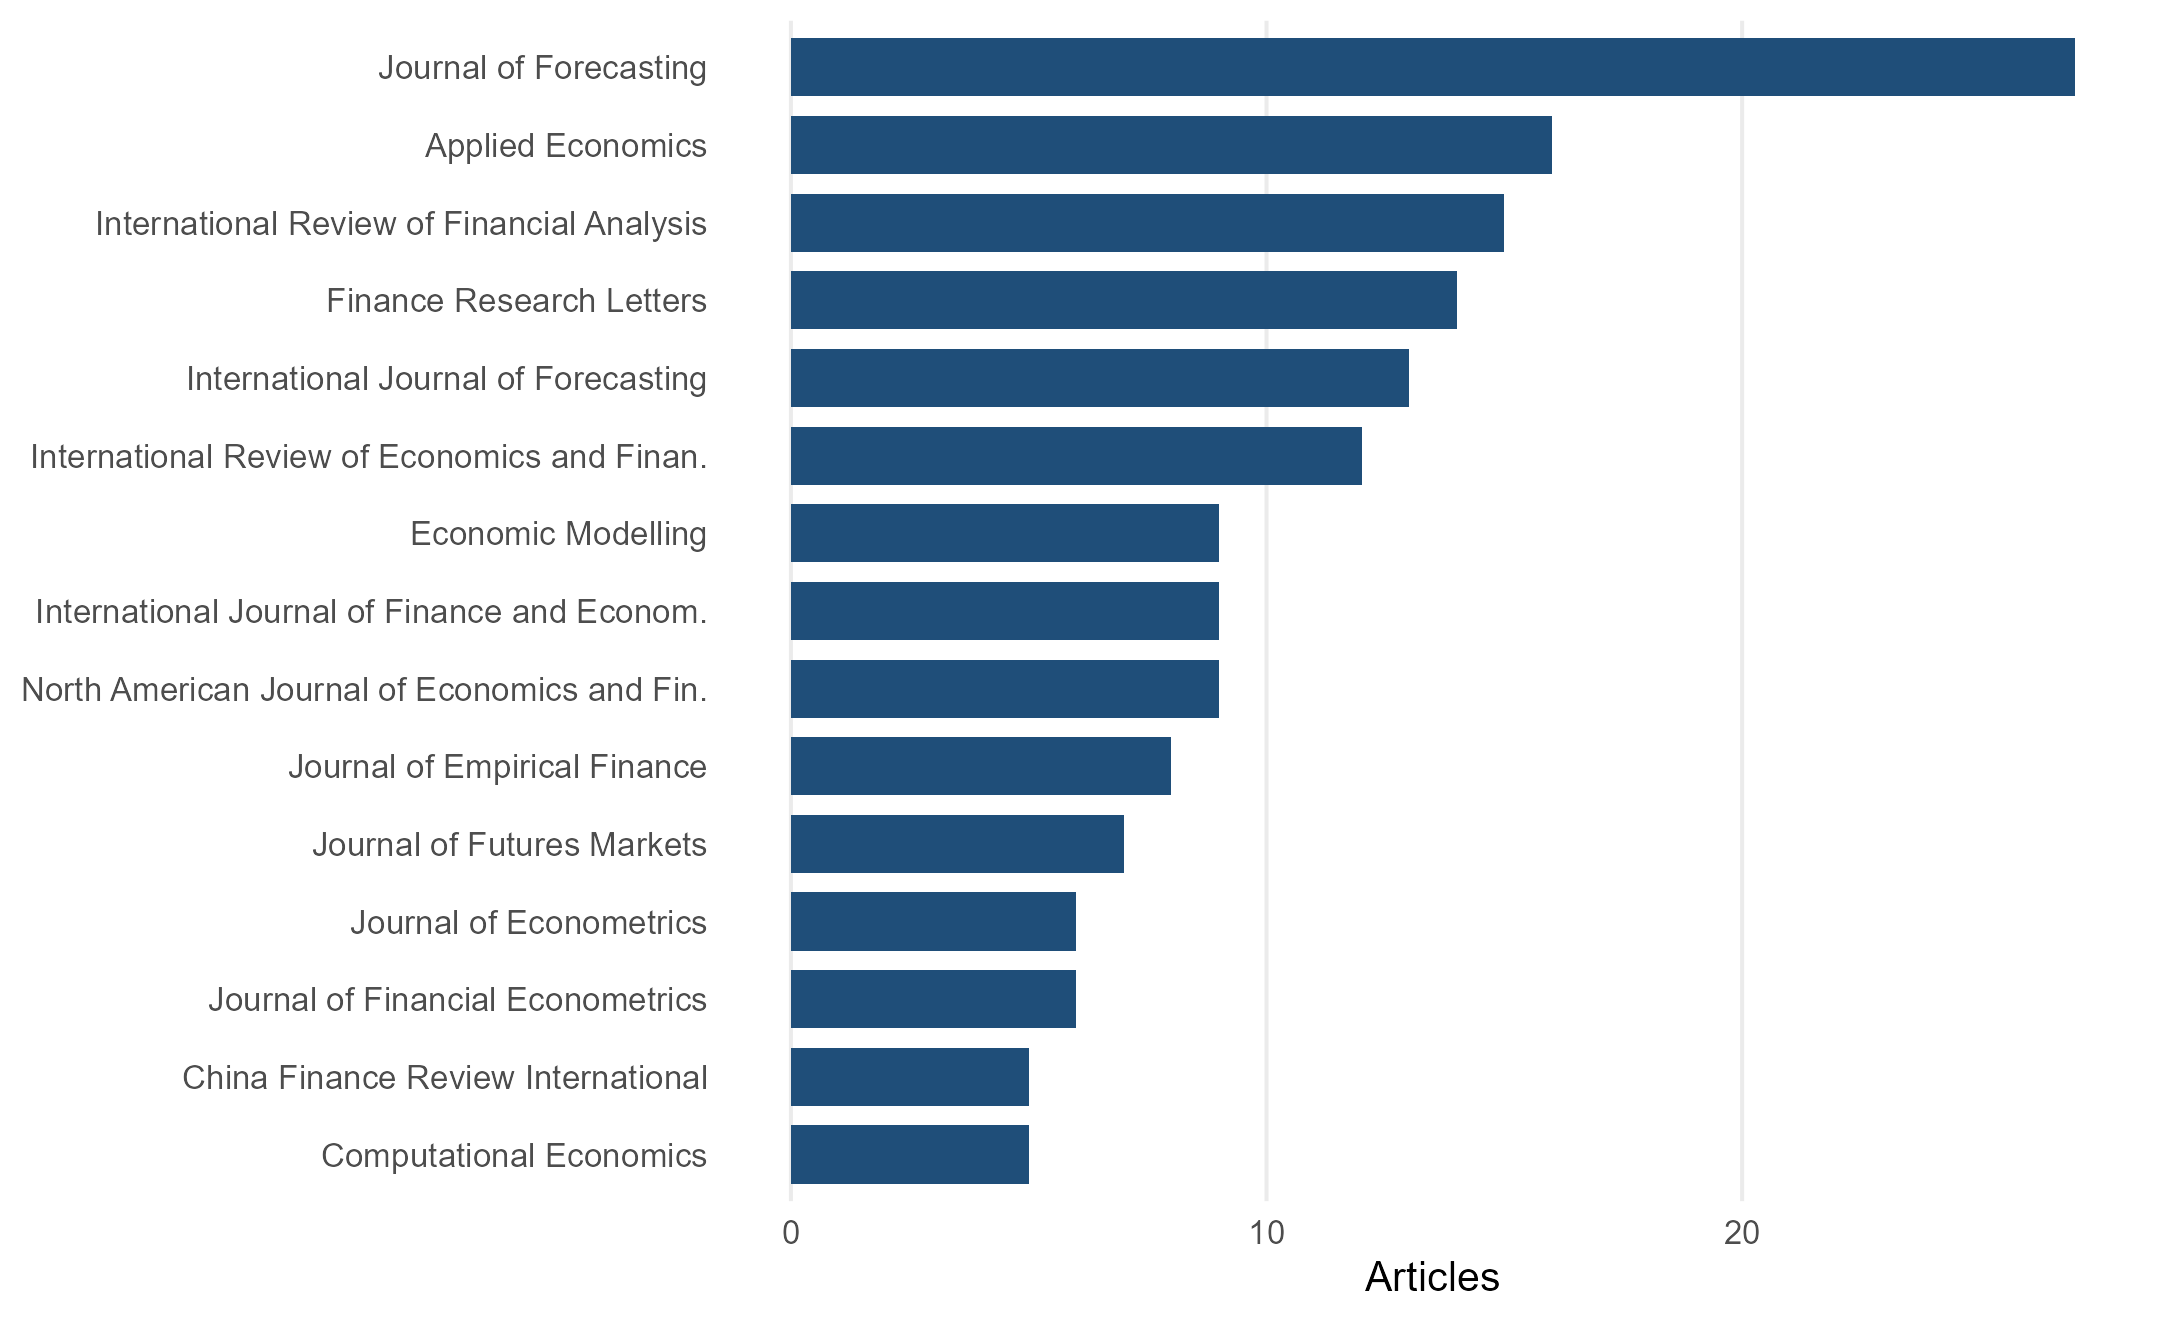
\includegraphics[width=0.86\linewidth]{figures/lit_sources.png}
\caption{Most productive sources}
\end{subfigure}
\begin{subfigure}{\linewidth}\centering
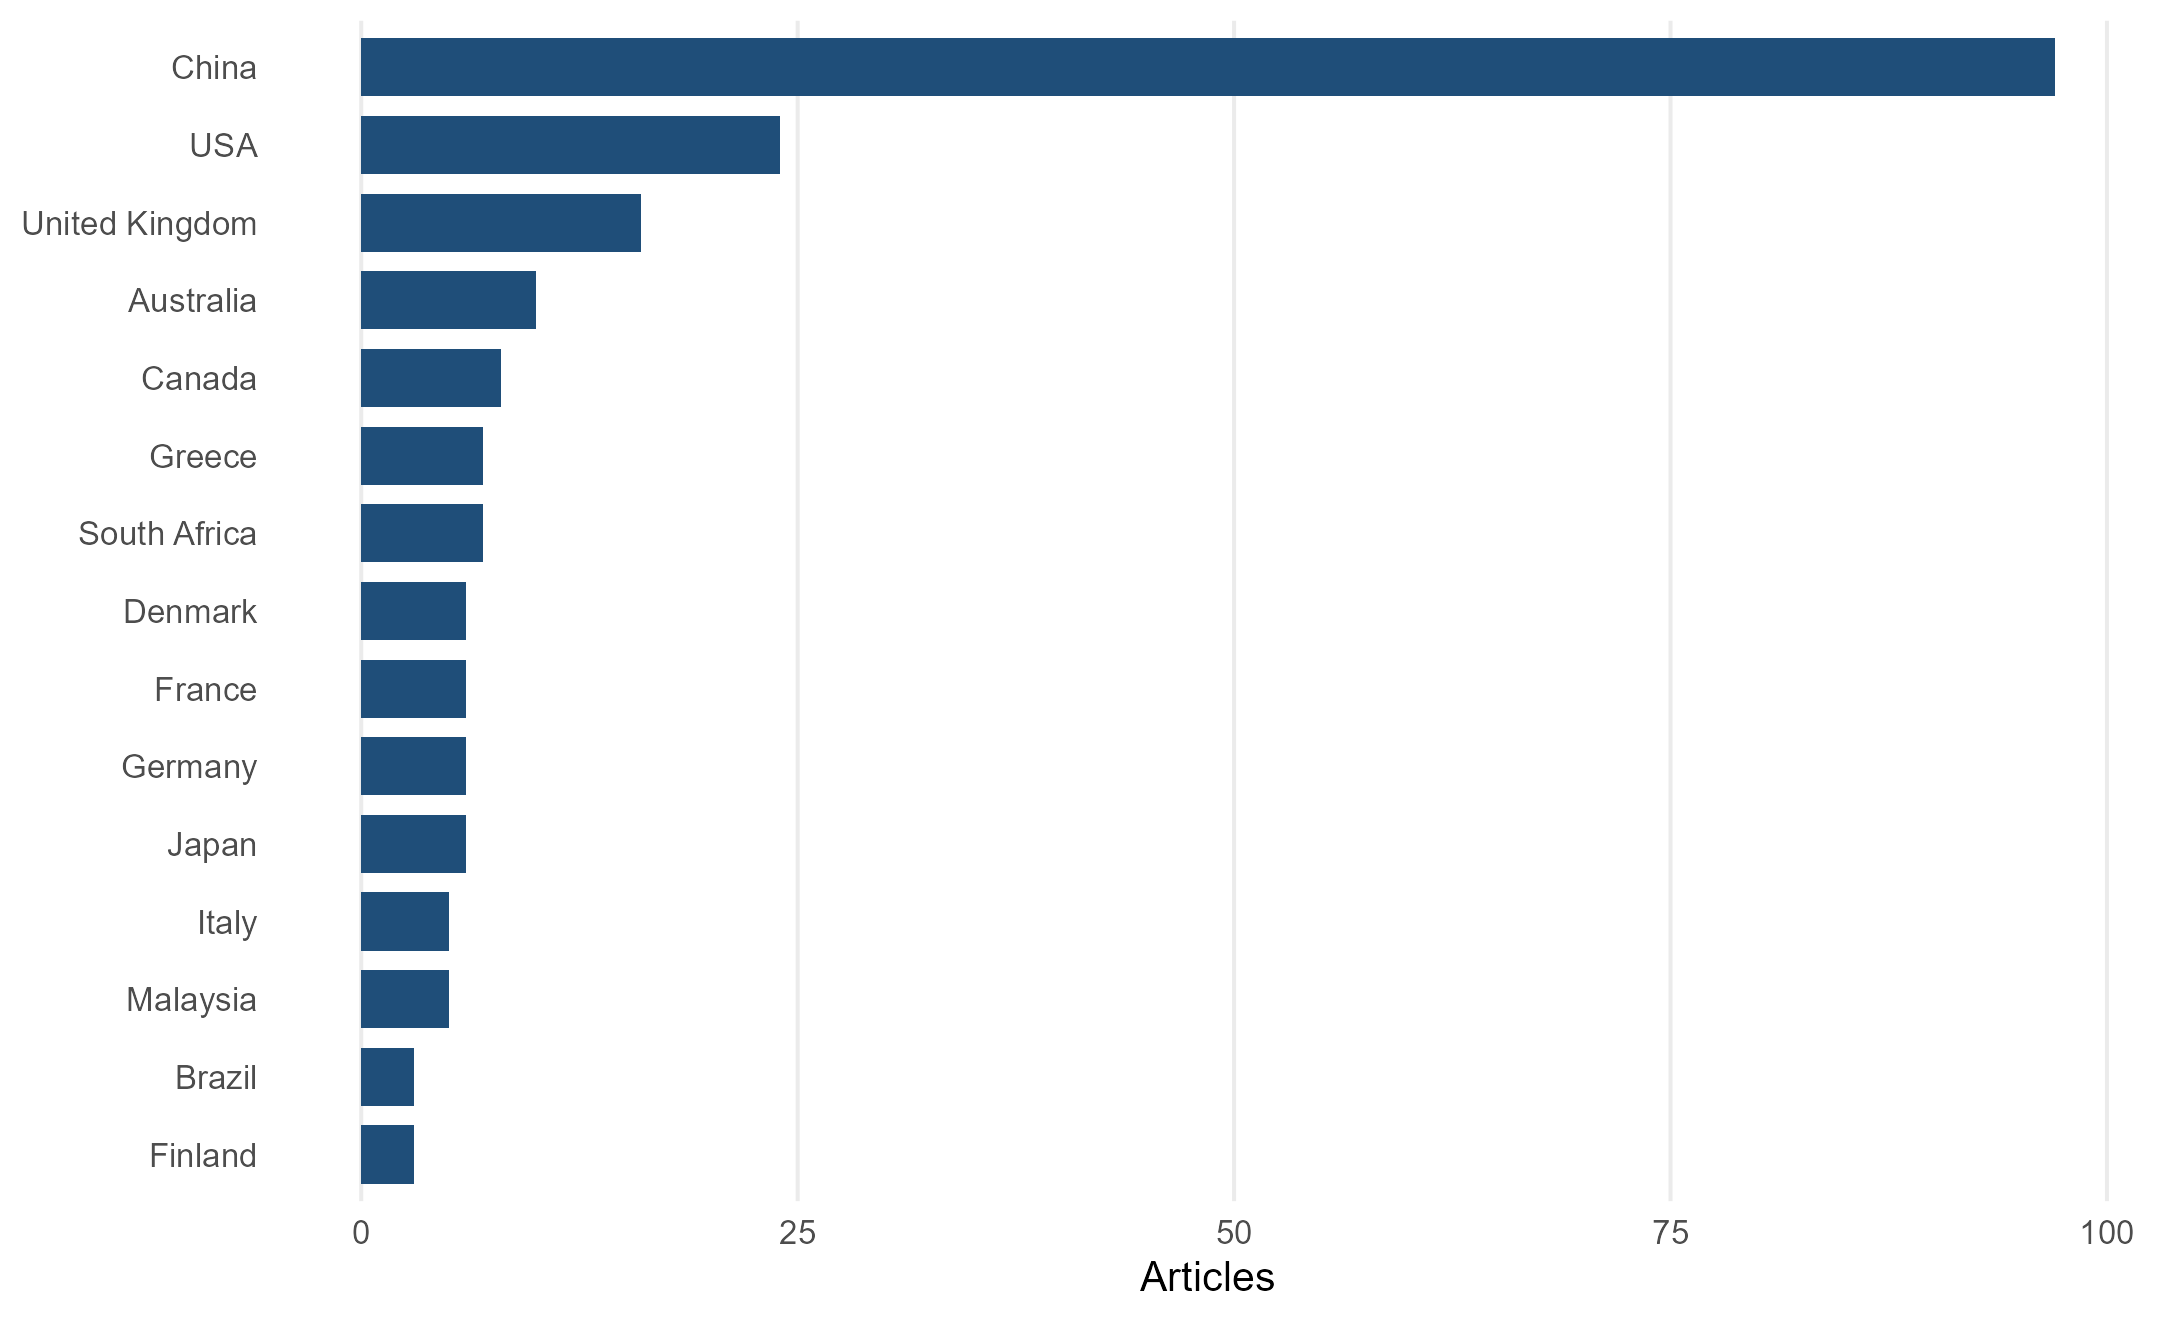
\includegraphics[width=0.86\linewidth]{figures/lit_countries.png}
\caption{Corresponding-author country}
\end{subfigure}
\label{fig:litproduction}
\end{figure}
